\documentclass[12pt]{report}
\usepackage[a4paper]{geometry}
\usepackage[myheadings]{fullpage}
\usepackage{fancyhdr}
\usepackage{lastpage}
\usepackage{graphicx, wrapfig, subcaption, setspace, booktabs}
\usepackage[T1]{fontenc}
\usepackage[font=small, labelfont=bf]{caption}
\usepackage{fourier}
\usepackage[protrusion=true, expansion=true]{microtype}
\usepackage[english]{babel}
\usepackage{sectsty}
\usepackage{url, lipsum}
\usepackage[color]{vdmlisting}
\usepackage[hidelinks]{hyperref} 
\usepackage{longtable}
\usepackage[utf8]{inputenc}
\usepackage{graphicx}
\graphicspath{ {images/} }

\newcommand{\HRule}[1]{\rule{\linewidth}{#1}}
\onehalfspacing
\setcounter{tocdepth}{5}
\setcounter{secnumdepth}{5}

\lstdefinestyle{DOS}
{
    backgroundcolor=\color{black},
    basicstyle=\scriptsize\color{white}\ttfamily
}

%-------------------------------------------------------------------------------
% HEADER & FOOTER
%-------------------------------------------------------------------------------
\pagestyle{fancy}
\fancyhf{}
\setlength\headheight{15pt}
\fancyhead[L]{MFES}
\fancyhead[R]{FEUP}
\fancyfoot[R]{\thepage\ }
%-------------------------------------------------------------------------------
% TITLE PAGE
%-------------------------------------------------------------------------------

\begin{document}

\title{ \normalsize \textsc{Métodos Formais em Engenharia de Software}
		\\ [2.0cm]
		\HRule{0.5pt} \\
		\LARGE \textbf{\uppercase{Formal Modeling of a Parking Lot Management System in VDM++}}
		\HRule{2pt} \\ [0.5cm]
		\normalsize \today \vspace*{5\baselineskip}}

\date{}

\author{
		Ricardo Manuel Correia Magalhães \\ 
		Mestrado Integrado em Engenharia Informática e de Computação \\
		Faculdade de Engenharia da Universidade do Porto }

\maketitle
\tableofcontents
\newpage

%-------------------------------------------------------------------------------
% Section title formatting
\sectionfont{\scshape}
%-------------------------------------------------------------------------------

%-------------------------------------------------------------------------------
% BODY
%-------------------------------------------------------------------------------

\section*{1. Informal system description and list of requirements}
\addcontentsline{toc}{section}{1. Informal system description and list of requirements}
\subsection*{1.1. Informal system description}
\addcontentsline{toc}{subsection}{1.1. Informal system description}

This system's goal is to maintain a set of parking lots. The users have a card with information (expiration date, plates, etc) and can enter or leave parking lots authorized for their group. The system is capable of creating every entity (card, parking, group) and doing operations, allowing or denying it. It can also list operations of a certain card and canceling or reactivating it.

\subsection*{1.2. List of requirements}
\addcontentsline{toc}{subsection}{1.2. List of requirements}

\begin{longtable}{|c|c|c|}
\hline
\textbf{Id} & \textbf{Priority} & \textbf{Description} \\
\hline
R1 & Mandatory & Add groups to the system.\\
\hline
R2 & Mandatory & Add a card, along with its owner's name and plates, with the belonging group.\\
\hline
R3 & Mandatory & Add a parking lot to be used by a certain group.\\
\hline
R4 & Mandatory & Add an operation (car entering or leaving). \\
\hline
R5 & Mandatory & List a card's operations.\\
\hline
R6 & Mandatory & Cancel and reactivate a card. \\
\hline
R6 & Mandatory & Check information about current parking lot's lotation. \\
\hline
\end{longtable}

\newpage

\section*{2. Visual UML Model}
\addcontentsline{toc}{section}{2. Visual UML Model}
\subsection*{2.1. Use Case Model}
\addcontentsline{toc}{subsection}{2.1. Use Case Model}

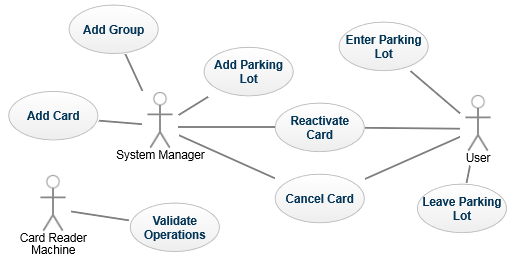
\includegraphics{use-case-model}

\subsection*{2.2. Class Model}
\addcontentsline{toc}{subsection}{2.2. Class Model}

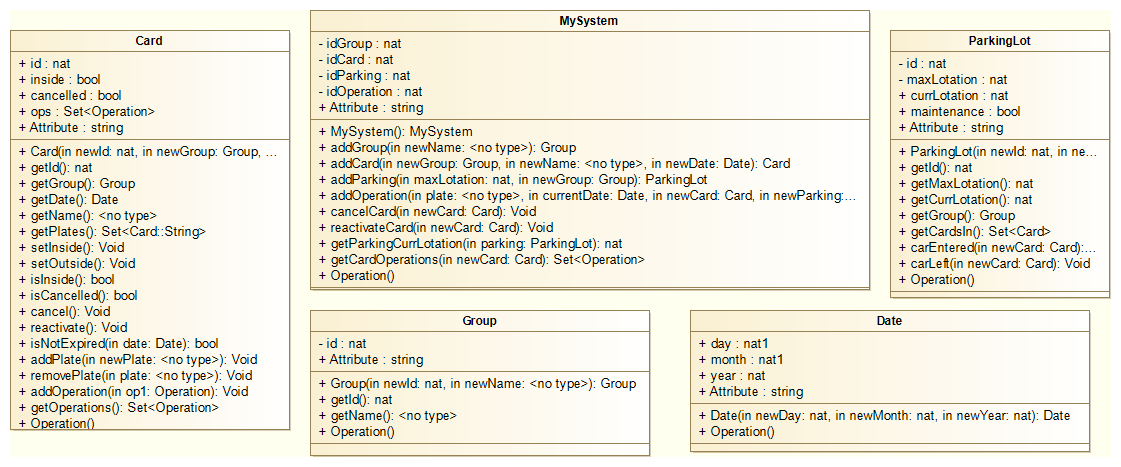
\includegraphics[width=\textwidth,height=\textheight,keepaspectratio]{mfes-class-diagram}

\begin{longtable}{|c|c|}
\hline
\textbf{Class Name} & \textbf{Description} \\
\hline
Card & Save card information and do operations related to it.\\
\hline
Group & Save group information and do operations related to it.\\
\hline
ParkingLot & Save parking lot information and do operations related to it.\\
\hline
Date & Auxiliar class to store date.\\
\hline
MySystem & Main class to do all operations \\
\hline
\end{longtable}

\newpage

\section*{3. Formal VDM++ Model}
\addcontentsline{toc}{section}{3. Formal VDM++ Model}

\subsection*{3.1. Card}
\addcontentsline{toc}{subsection}{3.1. Card}
\begin{vdmpp}[breaklines=true]
class Card

types
public String = seq of char;

instance variables
public id: nat;
public group: Group;
public username: String;
public plates: set of String;
public inside: bool;
public expirationDate: Date;
public cancelled: bool;
public ops: set of Operation;

operations
(*@
\label{Card:17}
@*)
public Card: nat*Group*String*Date==> Card
 Card(newId,newGroup,newName,newDate) == (
  id := newId;
  group := newGroup;
  username := newName;
  plates := {};
  inside := false;
  expirationDate := newDate;
  cancelled := false;
  ops := {};
  return self;
 );
 
(*@
\label{getId:30}
@*)
public getId: () ==> nat
 getId() == return self.id;
 
(*@
\label{getGroup:33}
@*)
public getGroup: () ==> Group
 getGroup() == return self.group;
 
(*@
\label{getDate:36}
@*)
public getDate: () ==> Date
 getDate() == return self.expirationDate;
 
(*@
\label{getName:39}
@*)
public getName: () ==> String
 getName() == return self.username;

(*@
\label{getPlates:42}
@*)
public getPlates: () ==> set of String
 getPlates() == return self.plates;
 
(*@
\label{setInside:45}
@*)
public setInside: () ==> ()
 setInside() == inside := true;
 
(*@
\label{setOutside:48}
@*)
public setOutside: () ==> ()
 setOutside() == inside := false; 
 
(*@
\label{isInside:51}
@*)
public isInside: () ==> bool
 isInside() == return self.inside;
 
(*@
\label{isCancelled:54}
@*)
public isCancelled: () ==> bool
 isCancelled() == return self.cancelled;
 
(*@
\label{cancel:57}
@*)
public cancel: () ==> ()
 cancel() == cancelled := true;
 
(*@
\label{reactivate:60}
@*)
public reactivate: () ==> ()
 reactivate() == cancelled := false;
 
(*@
\label{isNotExpired:63}
@*)
public isNotExpired: (Date) ==> bool
 isNotExpired(date) == (
  if expirationDate.year > date.year or
  (expirationDate.year = date.year and (*@\vdmnotcovered{expirationDate}@*).(*@\vdmnotcovered{month}@*) (*@\vdmnotcovered{>}@*) (*@\vdmnotcovered{date}@*).(*@\vdmnotcovered{month}@*)) or
  (expirationDate.year = date.year and (*@\vdmnotcovered{expirationDate}@*).(*@\vdmnotcovered{month}@*) (*@\vdmnotcovered{=}@*) (*@\vdmnotcovered{date}@*).(*@\vdmnotcovered{month}@*)
   (*@\vdmnotcovered{and}@*) (*@\vdmnotcovered{expirationDate}@*).(*@\vdmnotcovered{day}@*) (*@\vdmnotcovered{>=}@*) (*@\vdmnotcovered{date}@*).(*@\vdmnotcovered{day}@*))
  then (*@\vdmnotcovered{return}@*) (*@\vdmnotcovered{true}@*)
  else return false;
 );
 
 
(*@
\label{addPlate:74}
@*)
public addPlate: String ==> ()
 addPlate(newPlate) == (
  plates := plates union {newPlate}
 )
 pre newPlate not in set plates;

(*@
\label{removePlate:80}
@*)
public removePlate: String ==> ()
 removePlate(plate) == (
  plates := plates \ {plate}
 )
 pre plate in set plates;
 
(*@
\label{addOperation:86}
@*)
public addOperation: Operation ==> ()
 addOperation(op1) == (
  ops := ops union {op1}
 );
 
(*@
\label{getOperations:91}
@*)
public getOperations: () ==> set of Operation
 getOperations() == return self.ops;
 
end Card
\end{vdmpp}
\bigskip
\begin{longtable}{|l|r|r|r|}
\hline
Function or operation & Line & Coverage & Calls \\
\hline
\hline
\hyperref[Card:17]{Card} & 17&100.0\% & 3 \\
\hline
\hyperref[addOperation:86]{addOperation} & 86&100.0\% & 3 \\
\hline
\hyperref[addPlate:74]{addPlate} & 74&100.0\% & 2 \\
\hline
\hyperref[cancel:57]{cancel} & 57&100.0\% & 1 \\
\hline
\hyperref[getDate:36]{getDate} & 36&100.0\% & 1 \\
\hline
\hyperref[getGroup:33]{getGroup} & 33&100.0\% & 1 \\
\hline
\hyperref[getId:30]{getId} & 30&100.0\% & 1 \\
\hline
\hyperref[getName:39]{getName} & 39&100.0\% & 1 \\
\hline
\hyperref[getOperations:91]{getOperations} & 91&100.0\% & 1 \\
\hline
\hyperref[getPlates:42]{getPlates} & 42&100.0\% & 2 \\
\hline
\hyperref[isCancelled:54]{isCancelled} & 54&100.0\% & 3 \\
\hline
\hyperref[isInside:51]{isInside} & 51&100.0\% & 3 \\
\hline
\hyperref[isNotExpired:63]{isNotExpired} & 63&56.0\% & 1 \\
\hline
\hyperref[reactivate:60]{reactivate} & 60&100.0\% & 1 \\
\hline
\hyperref[removePlate:80]{removePlate} & 80&100.0\% & 1 \\
\hline
\hyperref[setInside:45]{setInside} & 45&100.0\% & 1 \\
\hline
\hyperref[setOutside:48]{setOutside} & 48&100.0\% & 1 \\
\hline
\hline
Card.vdmpp & & 84.4\% & 27 \\
\hline
\end{longtable}


\subsection*{3.2. Date}
\addcontentsline{toc}{subsection}{3.2. Date}
\begin{vdmpp}[breaklines=true]
class Date

instance variables
public day: nat1;
public month: nat1;
public year: nat;

operations
(*@
\label{Date:9}
@*)
public Date: nat*nat*nat ==> Date
 Date(newDay,newMonth,newYear) == (
  day := newDay;
  month := newMonth;
  year := newYear;
 )
 pre newDay < 32 and newMonth < 13;
 
end Date
\end{vdmpp}
\bigskip
\begin{longtable}{|l|r|r|r|}
\hline
Function or operation & Line & Coverage & Calls \\
\hline
\hline
\hyperref[Date:9]{Date} & 9&100.0\% & 5 \\
\hline
\hline
Date.vdmpp & & 100.0\% & 5 \\
\hline
\end{longtable}


\subsection*{3.3. Group}
\addcontentsline{toc}{subsection}{3.3. Group}
\begin{vdmpp}[breaklines=true]
class Group

types
public String = seq of char;

instance variables
id: nat;
name: String;

operations

(*@
\label{Group:12}
@*)
public Group: nat*String ==> Group
 Group(newId,newName) == (
  id := newId;
  name := newName;
  return self;
 );
 
(*@
\label{getId:19}
@*)
public getId: () ==> nat
 getId() == return self.id;
 
(*@
\label{getName:22}
@*)
public getName: () ==> String
 getName() == return self.name;

end Group
\end{vdmpp}
\bigskip
\begin{longtable}{|l|r|r|r|}
\hline
Function or operation & Line & Coverage & Calls \\
\hline
\hline
\hyperref[Group:12]{Group} & 12&100.0\% & 3 \\
\hline
\hyperref[getId:19]{getId} & 19&100.0\% & 1 \\
\hline
\hyperref[getName:22]{getName} & 22&100.0\% & 2 \\
\hline
\hline
Group.vdmpp & & 100.0\% & 6 \\
\hline
\end{longtable}


\subsection*{3.4. MySystem}
\addcontentsline{toc}{subsection}{3.4. MySystem}
\begin{vdmpp}[breaklines=true]
class MySystem
types
public String = seq of char;
public Result = <Allow> | <Deny>;
public Type = <Enter> | <Leave>;

instance variables
idGroup: nat;
idCard: nat;
idParking: nat;
idOperation: nat;

groups: set of Group;
cards: set of Card;
parkings: set of ParkingLot;
ops: set of Operation;

operations
(*@
\label{MySystem:19}
@*)
(*@
\label{System:19}
@*)
(*@
\label{MySystem:19}
@*)
(*@
\label{System:19}
@*)
public MySystem: () ==> MySystem
 MySystem() == (
  idGroup:=0;
  idCard:=0;
  idParking:=0;
  idOperation:=0;
  groups := {};
  cards := {};
  parkings := {};
  ops := {};
  return self;
 );
 
(*@
\label{addGroup:32}
@*)
(*@
\label{addGroup:32}
@*)
(*@
\label{addGroup:32}
@*)
public addGroup: String ==> Group
 addGroup(newName) == (
  dcl newGroup: Group := new Group(idGroup,newName);
  groups := groups union {newGroup};
  idGroup := idGroup + 1;
  return newGroup;
 );
 
(*@
\label{addCard:40}
@*)
(*@
\label{addCard:40}
@*)
(*@
\label{addCard:40}
@*)
public addCard: Group*String*Date==> Card
 addCard(newGroup,newName,newDate) == (
  dcl newCard: Card := new Card(idCard,newGroup,newName,newDate);
  cards := cards union {newCard};
  idCard := idCard+1;
  return newCard;
 )
 pre newGroup in set groups;
 
(*@
\label{addParking:49}
@*)
(*@
\label{addParking:49}
@*)
(*@
\label{addParking:49}
@*)
public addParking: nat*Group ==> ParkingLot
 addParking(maxLotation,newGroup) == (
  dcl newParking: ParkingLot := new ParkingLot(idParking,maxLotation,newGroup);
  parkings := parkings union {newParking};
  idParking := idParking + 1;
  return newParking;
 )
 pre newGroup in set groups;
 
(*@
\label{addOperation:58}
@*)
(*@
\label{addOperation:58}
@*)
(*@
\label{addOperation:58}
@*)
public addOperation: String*Date*Card*ParkingLot*Type ==> Operation
 addOperation(plate,currentDate,newCard,newParking,newType) == (
  dcl newOp: Operation := new Operation(idOperation,currentDate,newCard,newParking,newType);
  ops := ops union {newOp};
  return newOp;
 )
 pre newCard in set cards and newParking in set parkings and plate in set newCard.plates;
 
(*@
\label{cancelCard:66}
@*)
(*@
\label{cancelCard:66}
@*)
(*@
\label{cancelCard:66}
@*)
public cancelCard: Card ==> ()
 cancelCard(newCard) == (
  newCard.cancel()
 )
 pre newCard in set cards
 post newCard.cancelled = true;

(*@
\label{reactivateCard:73}
@*)
(*@
\label{reactivateCard:73}
@*)
(*@
\label{reactivateCard:73}
@*)
public reactivateCard: Card ==> ()
 reactivateCard(newCard) == (
  newCard.reactivate()
 )
 pre newCard in set cards
 post newCard.cancelled = false;

(*@
\label{getParkingCurrLotation:80}
@*)
(*@
\label{getParkingCurrLotation:80}
@*)
(*@
\label{getParkingCurrLotation:80}
@*)
public getParkingCurrLotation: ParkingLot ==> nat
 getParkingCurrLotation(parking) == (
  return parking.getCurrLotation();
 )
 pre parking in set parkings;
 
(*@
\label{getCardOperations:86}
@*)
(*@
\label{getCardOperations:86}
@*)
(*@
\label{getCardOperations:86}
@*)
public getCardOperations: Card ==> set of Operation
 getCardOperations(newCard) == (return newCard.getOperations())
 pre newCard in set cards;

end MySystem
\end{vdmpp}
\bigskip
\begin{longtable}{|l|r|r|r|}
\hline
Function or operation & Line & Coverage & Calls \\
\hline
\hline
\hyperref[MySystem:19]{MySystem} & 19&100.0\% & 3 \\
\hline
\hyperref[System:19]{System} & 19&100.0\% & 3 \\
\hline
\hyperref[addCard:40]{addCard} & 40&100.0\% & 3 \\
\hline
\hyperref[addGroup:32]{addGroup} & 32&100.0\% & 3 \\
\hline
\hyperref[addOperation:58]{addOperation} & 58&100.0\% & 3 \\
\hline
\hyperref[addParking:49]{addParking} & 49&100.0\% & 2 \\
\hline
\hyperref[cancelCard:66]{cancelCard} & 66&100.0\% & 1 \\
\hline
\hyperref[getCardOperations:86]{getCardOperations} & 86&100.0\% & 1 \\
\hline
\hyperref[getParkingCurrLotation:80]{getParkingCurrLotation} & 80&100.0\% & 1 \\
\hline
\hyperref[reactivateCard:73]{reactivateCard} & 73&100.0\% & 1 \\
\hline
\hline
MySystem.vdmpp & & 100.0\% & 57 \\
\hline
\end{longtable}


\subsection*{3.5. Operation}
\addcontentsline{toc}{subsection}{3.5. Operation}
\begin{vdmpp}[breaklines=true]
class Operation

types

public Result = <Allow> | <Deny>;
public Type = <Enter> | <Leave>;

instance variables

id: nat;
date: Date;
public cardUsed: Card;
parking: ParkingLot;
type: Type;
result: Result;

operations

(*@
\label{Operation:19}
@*)
public Operation: nat*Date*Card*ParkingLot*Type ==> Operation
 Operation(newId,newDate,newCard,newParking,newType) == (
  id := newId;
  date := newDate;
  cardUsed := newCard;
  parking := newParking;
  type := newType;
  
  if type = <Enter>
  then (*@\vdmnotcovered{self}@*).enter();
  
  if type = <Leave>
  then (*@\vdmnotcovered{self}@*).leave();
  
  cardUsed.addOperation(self);
  return self;
 );
 
(*@
\label{enter:37}
@*)
private enter: () ==> ()
 enter() == (
  result := <Deny>;
  if cardUsed not in set parking.getCardsIn() and not cardUsed.isInside()
  then (
  result := <Allow>;
  parking.carEntered(cardUsed);
  cardUsed.setInside();
  )
 ) 
 pre (cardUsed.expirationDate.year > date.year or --Check if it has not expired
  (cardUsed.expirationDate.year = date.year and cardUsed.expirationDate.month > date.month) or
  ((*@\vdmnotcovered{cardUsed}@*).(*@\vdmnotcovered{expirationDate}@*).(*@\vdmnotcovered{year}@*) (*@\vdmnotcovered{=}@*) (*@\vdmnotcovered{date}@*).(*@\vdmnotcovered{year}@*) (*@\vdmnotcovered{and}@*) (*@\vdmnotcovered{cardUsed}@*).(*@\vdmnotcovered{expirationDate}@*).(*@\vdmnotcovered{month}@*) (*@\vdmnotcovered{=}@*) (*@\vdmnotcovered{date}@*).(*@\vdmnotcovered{month}@*)
   (*@\vdmnotcovered{and}@*) (*@\vdmnotcovered{cardUsed}@*).(*@\vdmnotcovered{expirationDate}@*).(*@\vdmnotcovered{day}@*) (*@\vdmnotcovered{>=}@*) (*@\vdmnotcovered{date}@*).(*@\vdmnotcovered{day}@*)))
   and not cardUsed.cancelled --Check if card is cancelled
   and not parking.maintenance
   and not parking.currLotation = 0; --Check if parking is on maintenance;

(*@
\label{leave:55}
@*)
private leave: () ==> ()
 leave() == (
  result := <Deny>;
  if cardUsed in set parking.getCardsIn() and cardUsed.isInside()
  then (
  result := <Allow>;
  parking.carLeft(cardUsed);
  cardUsed.setOutside();
  )
 ); --I assumed not to check same things as in "enter" because the car has to go out even
   -- even if it is cancelled or expired, I guess
   
(*@
\label{getResult:67}
@*)
public getResult: () ==> Result
 getResult() == return self.result;

end Operation
\end{vdmpp}
\bigskip
\begin{longtable}{|l|r|r|r|}
\hline
Function or operation & Line & Coverage & Calls \\
\hline
\hline
\hyperref[Operation:19]{Operation} & 19&92.0\% & 3 \\
\hline
\hyperref[enter:37]{enter} & 37&72.6\% & 2 \\
\hline
\hyperref[getResult:67]{getResult} & 67&100.0\% & 3 \\
\hline
\hyperref[leave:55]{leave} & 55&100.0\% & 1 \\
\hline
\hline
Operation.vdmpp & & 81.3\% & 9 \\
\hline
\end{longtable}


\subsection*{3.6. ParkingLot}
\addcontentsline{toc}{subsection}{3.6. ParkingLot}
\begin{vdmpp}[breaklines=true]
class ParkingLot
types

instance variables
id: nat;
maxLotation: nat;
public currLotation: nat;
group: Group;
cardsIn: set of Card;
public maintenance: bool;

operations

(*@
\label{ParkingLot:14}
@*)
public ParkingLot: nat*nat*Group ==> ParkingLot
 ParkingLot(newId,newMaxLotation,newGroup) == (
  id := newId;
  maxLotation := newMaxLotation;
  currLotation := maxLotation;
  group := newGroup;
  cardsIn := {};
  maintenance := false;
  return self;
 );
 
(*@
\label{getId:25}
@*)
public getId: () ==> nat
 getId() == return self.id;
 
(*@
\label{getMaxLotation:28}
@*)
public getMaxLotation: () ==> nat
 getMaxLotation() == return self.maxLotation;
 
(*@
\label{getCurrLotation:31}
@*)
public getCurrLotation: () ==> nat
 getCurrLotation() == return self.currLotation;
 
(*@
\label{getGroup:34}
@*)
public getGroup: () ==> Group
 getGroup() == return self.group;
 
(*@
\label{getCardsIn:37}
@*)
public getCardsIn: () ==> set of Card
 getCardsIn() == return self.cardsIn;
 
(*@
\label{carEntered:40}
@*)
public carEntered: Card ==> ()
 carEntered(newCard) == (
  currLotation := currLotation-1;
  cardsIn := cardsIn union {newCard};
 );
 
(*@
\label{carLeft:46}
@*)
public carLeft: Card ==> ()
 carLeft(newCard) == (
  currLotation := currLotation+1;
  cardsIn := cardsIn \ {newCard};
 )
 post currLotation <= maxLotation;

end ParkingLot
\end{vdmpp}
\bigskip
\begin{longtable}{|l|r|r|r|}
\hline
Function or operation & Line & Coverage & Calls \\
\hline
\hline
\hyperref[ParkingLot:14]{ParkingLot} & 14&100.0\% & 2 \\
\hline
\hyperref[carEntered:40]{carEntered} & 40&100.0\% & 1 \\
\hline
\hyperref[carLeft:46]{carLeft} & 46&100.0\% & 1 \\
\hline
\hyperref[getCardsIn:37]{getCardsIn} & 37&100.0\% & 3 \\
\hline
\hyperref[getCurrLotation:31]{getCurrLotation} & 31&100.0\% & 2 \\
\hline
\hyperref[getGroup:34]{getGroup} & 34&100.0\% & 1 \\
\hline
\hyperref[getId:25]{getId} & 25&100.0\% & 1 \\
\hline
\hyperref[getMaxLotation:28]{getMaxLotation} & 28&100.0\% & 1 \\
\hline
\hline
ParkingLot.vdmpp & & 100.0\% & 12 \\
\hline
\end{longtable}



\newpage

\section*{4. Model Validation}
\addcontentsline{toc}{section}{4. Model Validation}

\subsection*{4.1.MyTestCase}
\addcontentsline{toc}{subsection}{4.1. MyTestCase}
\begin{vdmpp}[breaklines=true]
class MyTestCase
/*
  Superclass for test classes, simpler but more practical than VDMUnit`TestCase. 
  For proper use, you have to do: New -> Add VDM Library -> IO.
  FEUP, MFES, 2015/16.
*/

operations

 -- Simulates assertion checking by reducing it to pre-condition checking.
 -- If 'arg' does not hold, a pre-condition violation will be signaled.
(*@
\label{assertTrue:12}
@*)
 protected assertTrue: bool ==> ()
 assertTrue(arg) == 
  (*@\vdmnotcovered{return}@*) 
 pre (*@\vdmnotcovered{arg}@*);
  
 -- Simulates assertion checking by reducing it to post-condition checking.
 -- If values are not equal, prints a message in the console and generates 
 -- a post-conditions violation.
(*@
\label{assertEqual:20}
@*)
 protected assertEqual: ? * ? ==> ()
 assertEqual(expected, actual) == 
  if expected <> actual then (*@\vdmnotcovered{(}@*)
    (*@\vdmnotcovered{IO`print}@*)((*@\vdmnotcovered{"Actual value ("}@*));
    (*@\vdmnotcovered{IO`print}@*)((*@\vdmnotcovered{actual}@*)); 
    (*@\vdmnotcovered{IO`print}@*)((*@\vdmnotcovered{") different from expected ("}@*));
    (*@\vdmnotcovered{IO`print}@*)((*@\vdmnotcovered{expected}@*));
    (*@\vdmnotcovered{IO`println}@*)((*@\vdmnotcovered{")\textbackslash n"}@*))
  )
 post expected = actual
  
end MyTestCase
\end{vdmpp}
\bigskip
\begin{longtable}{|l|r|r|r|}
\hline
Function or operation & Line & Coverage & Calls \\
\hline
\hline
\hyperref[assertEqual:20]{assertEqual} & 20&38.8\% & 22 \\
\hline
\hyperref[assertTrue:12]{assertTrue} & 12&0.0\% & 0 \\
\hline
\hline
MyTestCase.vdmpp & & 35.0\% & 22 \\
\hline
\end{longtable}


\subsection*{4.2. Test}
\addcontentsline{toc}{subsection}{4.2. Test}
\begin{vdmpp}[breaklines=true]
class Test is subclass of MyTestCase

types
public Type = <Enter> | <Leave>;
public Result = <Allow> | <Deny>;

operations
(*@
\label{Test:8}
@*)
public Test: () ==> Test
 Test() == (
  return self;
  );
  
--Test initializing and populating MySystem.
(*@
\label{testMySystem:14}
@*)
(*@
\label{testSystem:14}
@*)
public testMySystem: () ==> ()
 testMySystem() == (
  dcl MySystem: MySystem := new MySystem();
  dcl group: Group := MySystem.addGroup("Students");
  dcl park: ParkingLot := MySystem.addParking(30,group);
  dcl date1: Date := new Date(31,12,2017);
  dcl card1: Card := MySystem.addCard(group,"John Doe",date1);
  
  assertEqual("Students",group.getName());
  assertEqual("Students",park.getGroup().getName());
  assertEqual(30,park.getMaxLotation());
  assertEqual("John Doe",card1.getName());
  assertEqual(group,card1.getGroup());
  assertEqual(date1,card1.getDate());
  
  assertEqual(0,group.getId());
  assertEqual(0,park.getId());
  assertEqual(0,card1.getId());
 );
 
(*@
\label{testCard:34}
@*)
public testCard: () ==> ()
 testCard() == (
  dcl MySystem: MySystem := new MySystem();
  dcl group: Group := MySystem.addGroup("Students");
  dcl date1: Date := new Date(1,1,2015);
  dcl date2: Date := new Date(2,2,2017);
  dcl card1: Card := MySystem.addCard(group,"John Doe",date1);
  
  assertEqual(false,card1.isCancelled());
  assertEqual(false,card1.isInside());
  assertEqual(false,card1.isNotExpired(date2));
  
  
  MySystem.cancelCard(card1);
  assertEqual(true,card1.isCancelled());
  
  MySystem.reactivateCard(card1);
  assertEqual(false,card1.isCancelled());
  
  card1.addPlate("33-MM-22");
  assertEqual({"33-MM-22"},card1.getPlates());
  card1.removePlate("33-MM-22");
  assertEqual({},card1.getPlates());
  
 );
 
 
(*@
\label{testOperation:61}
@*)
public testOperation: () ==> ()
 testOperation() == (
  dcl MySystem: MySystem := new MySystem();
  dcl group: Group := MySystem.addGroup("Students");
  dcl park1: ParkingLot := MySystem.addParking(30,group);
  dcl date1: Date := new Date(31,12,2017);
  dcl date2: Date := new Date(2,2,2017);
  dcl card1: Card := MySystem.addCard(group,"John Doe",date1);
  dcl op1: Operation;
  dcl op2: Operation;
  dcl op3: Operation;
  
  card1.addPlate("33-MM-22");
  op1 := MySystem.addOperation("33-MM-22",date2,card1,park1,<Enter>);
  op2 := MySystem.addOperation("33-MM-22",date2,card1,park1,<Enter>);
  
  assertEqual(<Allow>,op1.getResult());
  assertEqual(<Deny>,op2.getResult());
  assertEqual(29,MySystem.getParkingCurrLotation(park1));
  
  op3 := MySystem.addOperation("33-MM-22",date2,card1,park1,<Leave>);
  assertEqual(<Allow>,op1.getResult());
  assertEqual(30,park1.getCurrLotation());
  
  assertEqual({op1,op2,op3},MySystem.getCardOperations(card1));
  
 );
end Test
\end{vdmpp}
\bigskip
\begin{longtable}{|l|r|r|r|}
\hline
Function or operation & Line & Coverage & Calls \\
\hline
\hline
\hyperref[Test:8]{Test} & 8&100.0\% & 1 \\
\hline
\hyperref[testCard:34]{testCard} & 34&100.0\% & 1 \\
\hline
\hyperref[testMySystem:14]{testMySystem} & 14&100.0\% & 1 \\
\hline
\hyperref[testOperation:61]{testOperation} & 61&100.0\% & 1 \\
\hline
\hyperref[testSystem:14]{testSystem} & 14&100.0\% & 1 \\
\hline
\hline
Test.vdmpp & & 100.0\% & 5 \\
\hline
\end{longtable}



\newpage
\section*{5. Code Generation}
\addcontentsline{toc}{section}{5. Code Generation}
After successfully generating Java code, a console interface was built to test all the features. One of the things to change was 'seq of char' to 'String' in order to use the 'Scanner' class in Java. The interface is easy and minimalist, with menus navigation in lists with the option chosen by the user. Below are some examples.

\begin{lstlisting}[style=DOS]
**********
***MENU***
**********

1. Add Group
2. Add Card
3. Add Parking Lot
4. Register Operation
5. Get Card Operations
6. Cancel Card
7. Reactivate Card

Option: 1
\end{lstlisting}

\begin{lstlisting}[style=DOS]
**************
***ADD CARD***
**************

CHOOSE A GROUP FROM BELOW:

0. Students
Group ID: 0

------------------
Name: Ricardo
Day of Expiration Date: 1
Month of Expiration Date: 1
Year of Expiration Date: 2018
Add a Plate: 55-MM-FF

Press 1 to add another one; else to add the card as it is: 0
Card 'Ricardo' added!
Enter 0 for back menu...
\end{lstlisting}

\newpage
\section*{6. Conclusions}
\addcontentsline{toc}{section}{6. Conclusions}
The system does most of what is required, except renovating the expiration date of the card. Some more conditions and invariants could be added. Also, the class 'Date' should try to verify months with different number of days. However, the usage of VDM++ on this particular project contributed to my knowledge of the language and understanding the usefulness of it.

\newpage

\section*{7. References}
\addcontentsline{toc}{section}{7. References}
\begin{enumerate}
\item Class notes available in Moodle.
\item Overture IDE Guide.
\item \LaTeX\  documentation to write report.
\end{enumerate}




\end{document}